\setcounter{secnumdepth}{3}
\subsubsection{Model-View Controller}
Das Hauptmerkmal des Architekturmusters \ac{MVC} ist die Trennung der View und des Controllers. Genau das macht das MVC komfortabel f\"ur Web Anwendungen und weniger geeignet f\"ur Desktop Anwendungen\cite{Syromiatnikov2014}.

\subsubsection*{Model}
Das Model ist beim Architekturmuster \ac{MVC} der Ort, an dem die Daten und Objekte sowie der Netzwerkcode gespeichert und implementiert werden. Das hei\ss{}t, der Model Part beinhaltet die Informationen, um die View anschaulich zu machen und die Logik, die die \"Anderungen des Users verarbeitet und die View damit benachrichtigt\cite{Leff2001}.
\subsection*{View}
In der View ist ebenso wie in dem \ac{MVVM} Architekturmuster keinerlei Logik enthalten, was es wiederverwendbar f\"ur andere Projekte macht.\cite{Peres2016} Die View setzt Informationen f\"ur den Anwender ins Bild. Mit dem Controller zusammen definieren sie das User Interface (Benutzerschnittstelle)\cite{Leff2001}.
\subsection*{Controller}
Der Controller vermittelt vorwiegend \"uber \enquote{delegation pattern} zwischen der View und dem Model. Delegation Pattern ist eine Technik, bei der Objekte Verhalten nach au\ss{}en darlegen und das Verhaltens an ein anderes Objekt \"ubertragen\cite{TU-Wien2013}. Idealerwei\ss{}e kennt der Controller die View nicht und kommuniziert \"uber ein bestimmtes abstraktes Protokoll\cite{Peres2016}.
Der Controller verarbeitet die Events der View und leitet sie an das Model weiter, das dann die View \"uber die \"Anderung benachrichtigen kann und die View die \"Anderung dem Anwender darstellt. Vergleichbar mit dem ActionListener in Swing\cite{Singer2004}.
\subsection*{Model-View-Controller}
\begin{figure}[h] 
\centering
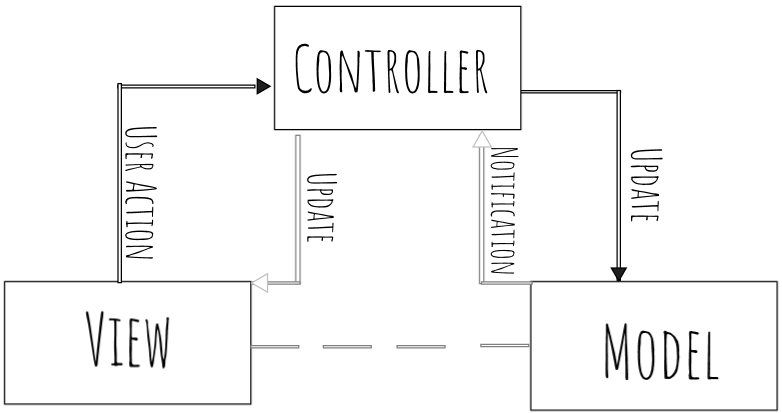
\includegraphics[scale=0.4]{fig/mvc.png} 
\caption{Komponente des MVC Architekturmusters}
\label{fig:MVC}
\end{figure} 
Auf Abbildung \ref{fig:MVC} erkennt man die Zusammenh\"ange zwischen den Komponenten des Architekturmodells \ac{MVC}. Dieses Modell l\"asst mehrere Views und Controller zu, die unabh\"angig von dem Model erstellt und modifiziert werden k\"onnen\cite{Curry2008}.
Wenn der Anwender eine Aktion in der View ausl\"ost, wird diese an den Controller geschickt, der anhand der Manipulation das Model aktualisiert. Sobald die Aktualisierung abgeschlossen ist, wird eine Benachrichtigung an den Controller gesendet, ob diese erfolgreich war oder nicht. War die Aktualisierung erfolgreich, aktualisiert der Controller anhand der Benachrichtigung die View.
\subsection*{Kommunikation}
Obwohl das Model unabh\"angig von den Views ist, sollten die Komponente miteinander kommunizieren. Ebenso die Controller und die Views. Da die View jedoch das Model kennt, kann die View mit dem Model in Kontakt treten. Die Kommunikation mit den Nachrichten findet \"uber \textbf{Events} (Aktionen) statt. Events stellen Mechanismen bereit, die mit wenigen Abh\"angigkeiten eine Kommunikation zustande kommen kann.
Grafische Komponente, wie Listen, Textfelder oder \"ahnliche k\"onnen Benachrichtigungen empfangen, beispielsweise wenn geklickt wird. Diese Benachrichtigungen kommen in der Regel vom Controller. Die View registrieren die Events an Objekte, die sie bearbeiten m\"ochten. Wenn die Nachricht zum Model gesendet wurde, wird das Application Model auf diese Nachricht antworten, die Daten aktualisieren und eine Nachricht zur\"uck senden. Das Application Model kann ebenso events ausl\"osen und somit die abh\"angigen Views \"uberwachen\cite{Deacon2005}. 
%F\"ur die Benachrichtigung vom Application Model zur View und umgekehrt ist der Controller zust\"andig, da der Controller die Anfragen des Anwenders interpretiert.

